\documentclass[conference]{IEEEtran}
\IEEEoverridecommandlockouts
% The preceding line is only needed to identify funding in the first footnote. If that is unneeded, please comment it out.
%Template version as of 6/27/2024

\usepackage{amsmath,amssymb,amsfonts}
\usepackage{algorithmic}
\usepackage{graphicx}
\usepackage{textcomp}
\usepackage{xcolor}
\usepackage[backend=biber,style=numeric]{biblatex}
\addbibresource{report.bib}

 \graphicspath{{assets/latex/}}

% Renders in red so unfinished sections are obvious. None may remain at submission.
\newcommand{\todo}[1]{\textcolor{red}{\textbf{TODO:} #1}}

\begin{document}

\title{CS6524 Computer Vision Lab. 1\\ Silhouettes and Fourier Epicycles}

\author{\IEEEauthorblockN{Darragh Luby}
\IEEEauthorblockA{\textit{University of Limerick}\\
23359048}
\and
\IEEEauthorblockN{Ellice Nelson}
\IEEEauthorblockA{\textit{University of Limerick}\\
23371323}
\and
\IEEEauthorblockN{Tóla Bowen MacCurtáin}
\IEEEauthorblockA{\textit{University of Limerick}\\
23383372}
\and
\IEEEauthorblockN{James Kelly}
\IEEEauthorblockA{\textit{University of Limerick}\\
23370858}
}

\maketitle

\begin{abstract}
\todo{The work done, the lessons learned, and the results, in a few words.}
\end{abstract}

\section{Methodology}

\subsection{Image Processing Pipeline}
\todo{Each step from raw image to boundary mask.}

\subsection{Silhouette Trajectory}
\todo{How edge pixels become an ordered, resampled curve, and any changes to the reference snippet.}

\subsection{Fourier Descriptors}
\todo{The 1D complex signal, the DFT, how the top $K$ harmonics are selected, and the reconstruction.}

\section{Justifications}

\subsection{Spatial Filters and Kernels}
\todo{Why these kernels and sizes? What did you try and reject?}

\subsection{Thresholding}
\todo{How were thresholds chosen? Which images needed their own values, and why?}

\section{Discussion and Failure Analysis}

\subsection{Results}
\todo{Where the pipeline succeeded or failed, per image, with figures from \texttt{out/}.}

\subsection{Improvements}
\todo{Concrete steps you would take with more time.}

% Figure example: copy the image from out/ into assets/latex/ first.
% Use figure* to span both columns.
%
% \begin{figure}
% \centerline{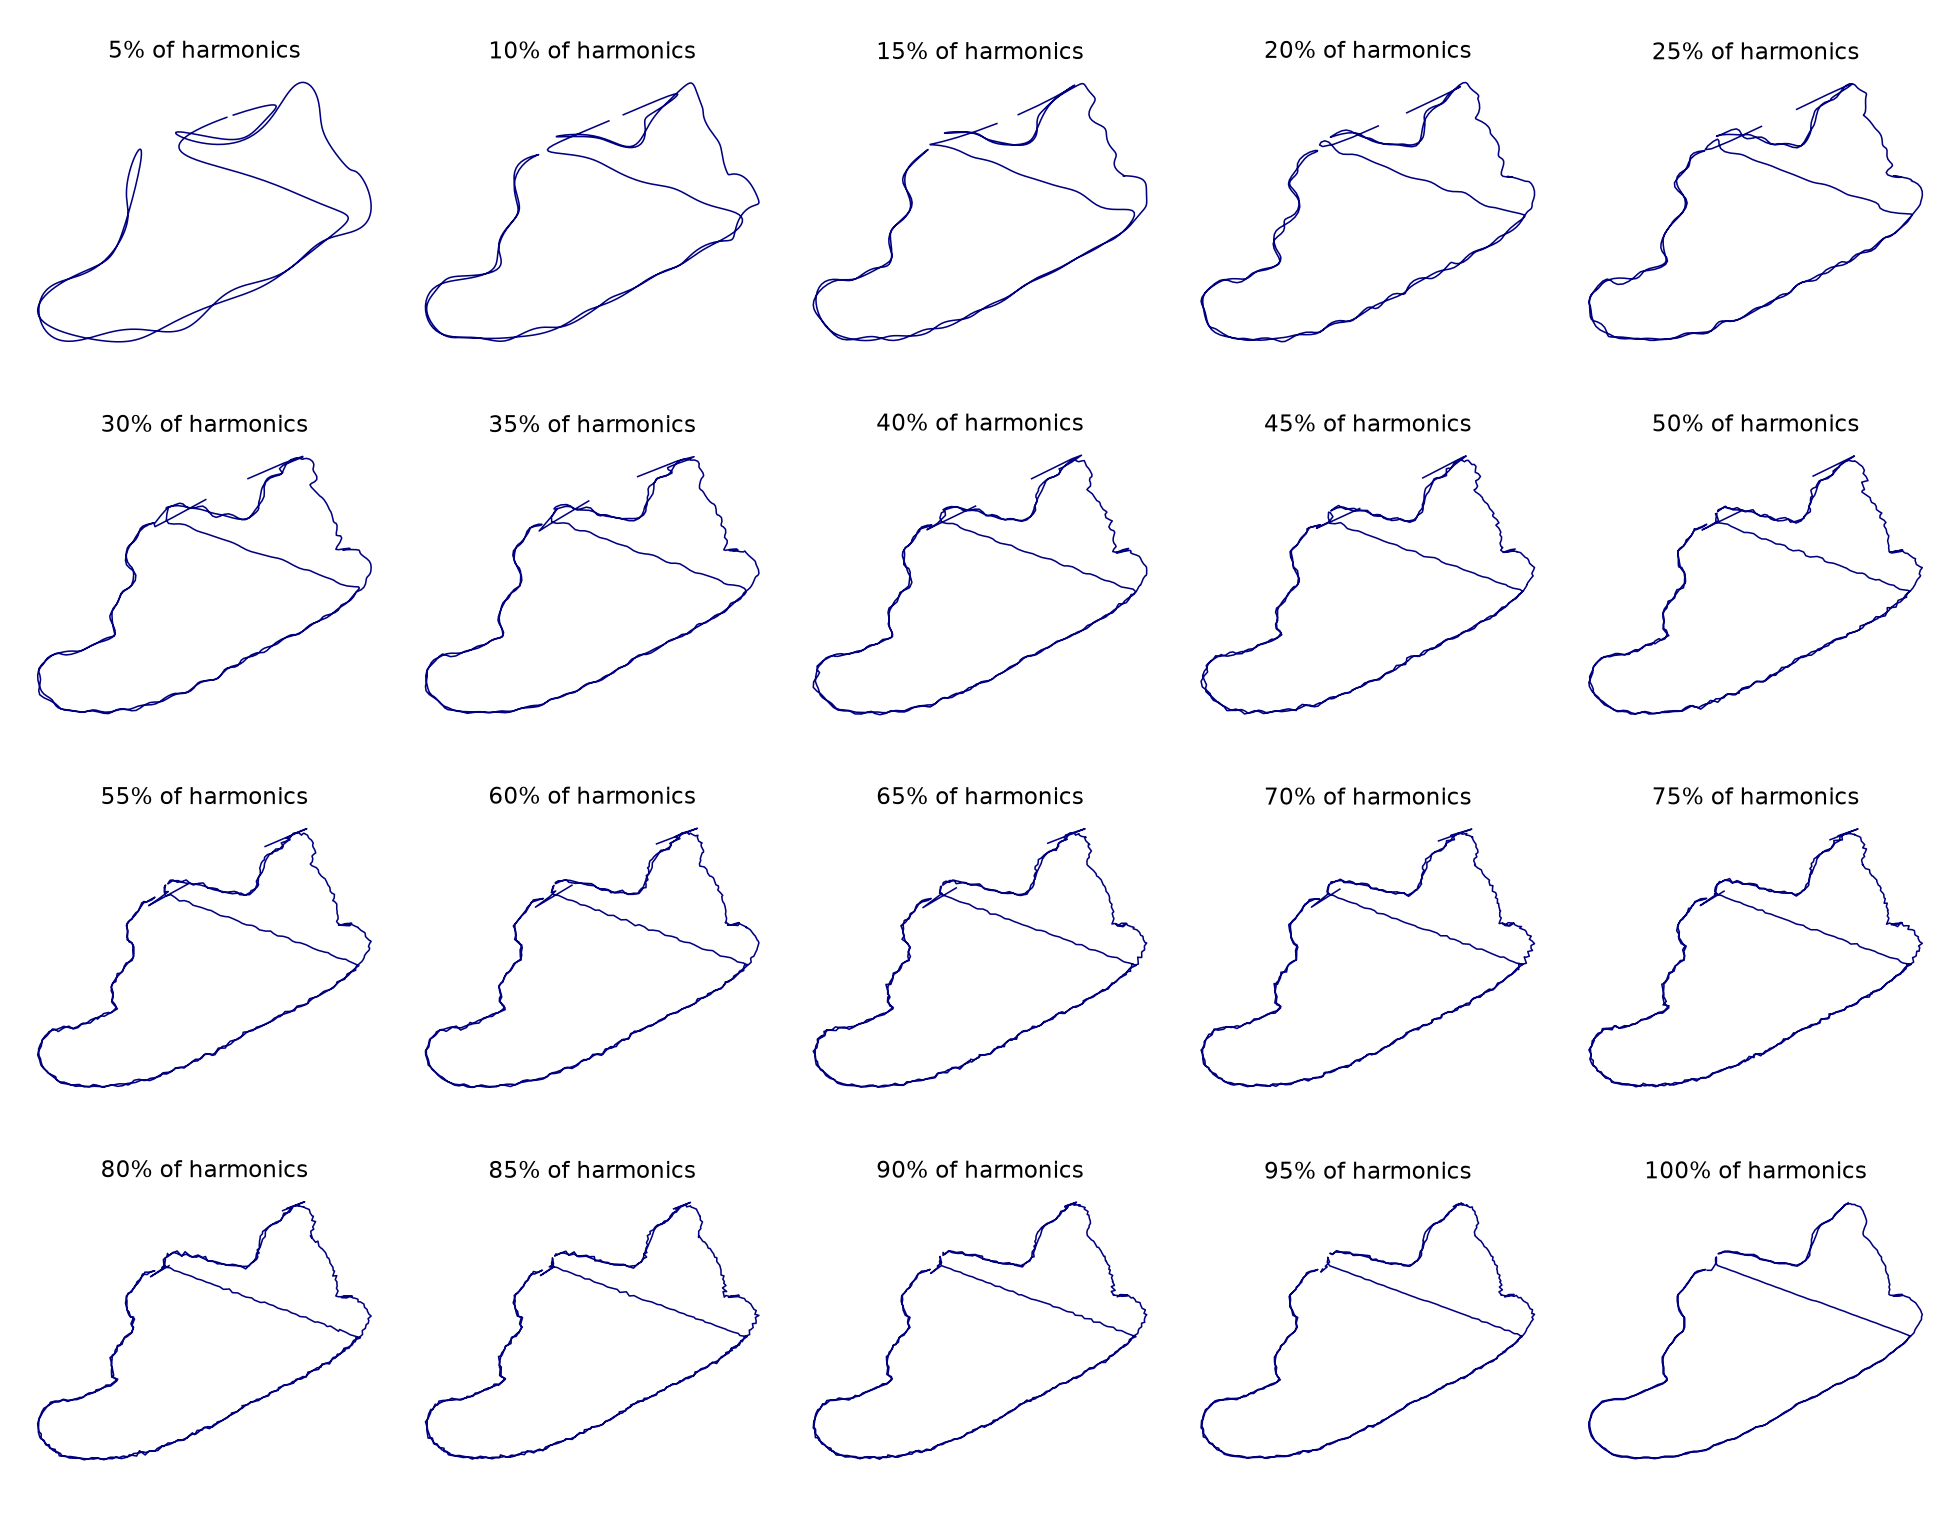
\includegraphics[width=\columnwidth]{00_final.png}}
% \caption{Reconstruction of image 00 with 5\% to 100\% of the harmonics.}
% \label{fig:final00}
% \end{figure}
%
% Reference it with Figure~\ref{fig:final00}. Cite sources from report.bib with \cite{foundationsCVbook}.

\printbibliography

\end{document}
